\documentclass{standalone}
\usepackage{pgfplots}
\usepackage{xcolor}
\definecolor{color1}{HTML}{FDB462}
\definecolor{color2}{HTML}{386CB0}
\definecolor{color3}{HTML}{40826D}

\begin{document}

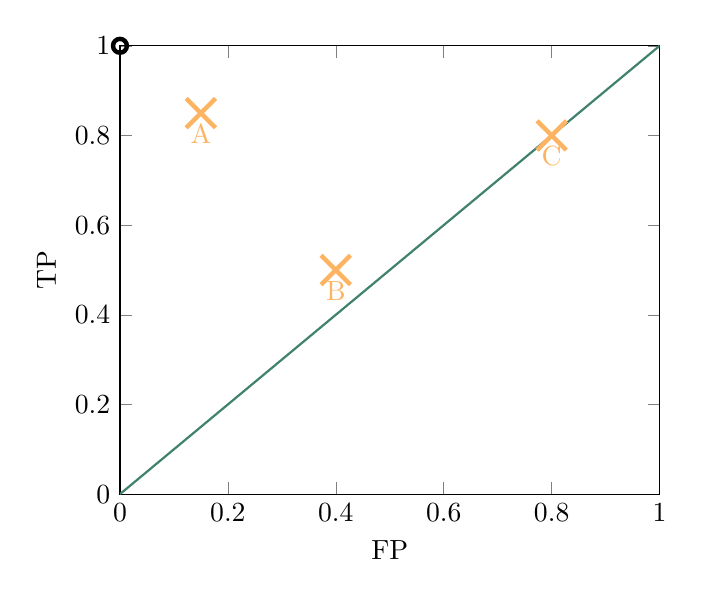
\begin{tikzpicture}
\begin{axis}[xlabel = FP, xmin = 0, xmax = 1, ylabel = TP, ymin = 0, ymax = 1]
\addplot[thick, mark = none, color = color3] coordinates{(0,0) (1,1)};
\addplot[color = color1, mark = x, mark size = 7.5pt, ultra thick] coordinates {(0.15,0.85)} node[below]{A};
\addplot[color = color1, mark = x, mark size = 7.5pt, ultra thick] coordinates {(0.4,0.5)} node[below]{B};
\addplot[color = color1, mark = x, mark size = 7.5pt, ultra thick] coordinates {(0.8,0.8)} node[below]{C};
\addplot[fill = color2, mark = o, mark size = 2.5, ultra thick] coordinates {(0,1)};
\end{axis}
\end{tikzpicture}
	
\end{document}
